% Prepared by Calvin Kent
%
% Assignment Template v19.02
%
%%% 20xx0x/MATHxxx/Crowdmark/Ax
%
\documentclass[12pt]{article} %
\usepackage{amsthm}
\usepackage{CKpreamble}
\usepackage{CKassignment}
\usepackage{mdframed}
\usepackage{euscript}
\usepackage{tikz}
\usepackage{pgfplots}

%
\begin{document}
	\pagenumbering{arabic}
	% Start of class settings ...
	\renewcommand*{\coursecode}{MATH 235} % renew course code
	\renewcommand*{\assgnnumber}{Assignment 1} % renew assignment number
	\renewcommand*{\submdate}{September 14, 2021} % renew the date
	\renewcommand*{\studentfname}{Abdullah} % Student first name
	\renewcommand*{\studentlname}{Zubair} % Student last name
    \renewcommand*{\proofname}{Proof:}
	% \renewcommand*{\studentnum}{20836288} % Student number

	\renewcommand\qedsymbol{$\blacksquare$}
	\setfigpath
	% End of class settings	
	% \pagestyle{crowdmark}
	\newgeometry{left=18mm, right=18mm, top=22mm, bottom=22mm} % page is set to default values
	\fancyhfoffset[L,O]{0pt} % header orientation fixed
	% End of class settings
	%%% Note to user:
	% CTRL + F <CHANGE ME:> (without the angular brackets) in CKpreamble to specify graphics paths accordingly.
	% The command \circled[]{} accepts one optional and one mandatory argument.
	% Optional argument is for the size of the circle and mandatory argument is for its contents.
	% \circled{A} produces circled A, with size drawn for letter A. \circled[TT]{A} produces circled A with size drawn for TT.
	% https://github.com/CalvinKent/My-LaTeX
	%%%

	%%%%%%%%%%%%%%%%%%%%%%%%%%%%%%%%%%%%%%%%%%%%%%%%%%%%%%%%%%%%%%%%%%%%%%%%%%%%%%%
	%%%                        CUSTOM MACRO VIM-TEX                             %%%
	%%       call IMAP('NOM', '\nomenclature{}', 'tex')               

	%%%%%%%%%%%%%%%%%%%%%%%%%%%%%%%%%%%%%%%%%%%%%%%%%%%%%%%%%%%%%%%%%%%%%%%%%%%%%%%

	% Crowdmark assignment start
	% qnumber, qname, points

\begin{center}
	\textbf{\underline{\Huge{Lecture 4 - Homework}}}
\end{center}

\begin{qstn}
 Suppose we have the identity function on $\R$, $\operatorname{id}_\R \colon \R \to \R$, $\operatorname{id}_\R(x) = x$. 
 Is it true that the inverse function of $\operatorname{id}_\R$ is itself? Justify your answer.
\end{qstn}

\begin{qstn}
  Let $ \mathcal{V} = \{1,4,9,25,49\} $ and $ \mathcal{W} = \{5,4,7,9,3\} $ be sets, define the following function, 
  \begin{itemize}
    \item $\mathcal{L} \colon \mathcal{V} \to \mathcal{W}$.
    \item $\mathcal{L}(v) = \sqrt{v} + 2$.
  \end{itemize}
  Prove that the function,
  \begin{itemize}
    \item $\mathcal{L}^{-1} \colon \mathcal{W} \to \mathcal{V}$.
    \item $\mathcal{L}^{-1}(w) = (w - 2)^2$.
  \end{itemize}
  is the inverse function for $\mathcal{L}$. 
\end{qstn}

\begin{qstn}
  Let $ \mathcal{V} = \{-1,0,1,5,8\} $ and $ \mathcal{W} = \{-3,0,1,4,5\} $ be sets, define the following function, 
  \begin{itemize}
    \item $\mathcal{T} \colon \mathcal{V} \to \mathcal{W}$.
    \item $\mathcal{T}(v) = \frac{3x}{x - 2}$.
  \end{itemize}
  Prove that the function,
  \begin{itemize}
    \item $\mathcal{T}^{-1} \colon \mathcal{W} \to \mathcal{V}$.
    \item $\mathcal{T}^{-1}(w) = \frac{2w}{w-3}$.
  \end{itemize}
  is the inverse function for $\mathcal{T}$. 
\end{qstn}

\begin{qstn}
  You are given the mapping diagram for a function $F \colon \mathcal{A} \to \mathcal{B}$. Your task is to determine the formula for the function as well as its
  inverse function based on the observed pattern.
    \begin{center}
     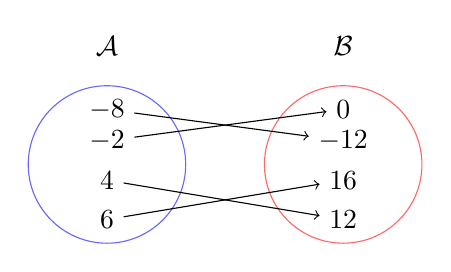
\begin{tikzpicture}
        % draw the sets
        \filldraw[fill=white!20, draw=blue!60] (-1.5,0) circle (1cm);
        \filldraw[fill=white!20, draw=red!60] (1.5,0) circle (1cm);


        % the texts
        \node at (-1.5,1.5) {$\mathcal{A}$};
        \node at (1.5,1.5) {$\mathcal{B}$};

        % the points in the sets (here I just create nodes to use them later on to position
        % the circles and the arrows
        \node (x1) at (-1.5,0.7) {$-8$};
        \node (x2) at (-1.5,0.3) {$-2$};
        \node (x3) at (-1.5,-0.2) {$4$};
        \node (x4) at (-1.5,-0.7) {$6$};
        \node (y1) at (1.5,0.7) {$0$};
        \node (y2) at (1.5,0.3) {$-12$};
        \node (y3) at (1.5,-0.2) {$16$};
        \node (y4) at (1.5,-0.7) {$12$};

        % draw the arrows
        \draw[->] (x1) -- (y2);
        \draw[->] (x2) -- (y1);
        \draw[->] (x3) -- (y4);
        \draw[->] (x4) -- (y3);

    \end{tikzpicture}
  \end{center}
\end{qstn}

\begin{qstn}
  Given an invertible function, can you explain why it would be advantageous to determine its inverse function?
  Why is it a useful tool? 
\end{qstn}

\begin{qstn}
  Let $f \colon \R \to \R$,  $f(x) = \left|x\right|$. Is $f$ invertible? If it is, prove it using mapping tables.
  If it is not, then provide a counter example to show that $f$ fails to be injective or surjective. (Its your choice)
  \textbf{(Important Question **)}.
\end{qstn}

\newpage

\begin{qstn}
  Let $G \colon \mathcal{A} \to \mathcal{B}$ be an invertible function. Suppose that the invertible function is,
  \[
      G^{-1}(b) = b - 2
  .\] 
  Given the co-domain $\mathcal{B} = \{-2,-1,0,3,7\} $ of $G$, recover the domain $\mathcal{A}$.
\end{qstn}


\begin{qstn}
  Given binary strings $\mathbf{S} = 00101$ and $\mathbf{T} = 1101$, determine the following,
  \begin{enumerate}[label=(\alph*)]
    \item $\mathbf{S} + \mathbf{T} + 0$.
    \item $1 + \mathbf{T} + 1$.
    \item $\epsilon + \mathbf{T} + \mathbf{S}$.
    \item $\mathbf{T} + \mathbf{T}$.
  \end{enumerate}
\end{qstn}

\begin{qstn}
  Recall that for normal addition of integers, $a + b = b + a$. Is this also true for binary strings? In other words is
  it always true that $\mathbf{S} + \mathbf{T} = \mathbf{T} + \mathbf{S}$? If it is, then prove it. If not, 
  then provide a counter example. 
\end{qstn}

\begin{qstn}
  Let $\mathbf{A} = 11011$. Determine,
  \begin{enumerate}[label=(\alph*)]
    \item The substring $\mathbf{R} = \vb a_1\vb a_3\vb a_5$.
    \item The substring $\mathbf{Z} = \vb a_1\vb a_2$.
    \item The substring $\mathbf{X} = \vb a_2\vb a_4$.
  \end{enumerate}
\end{qstn}

\begin{qstn}
Let $\EuScript{S} = \{11, 01, 10, 00\}$ and $\EuScript{R} = \{10001, 10101,11001,11101\} $. Define the following function,
  \begin{itemize}
    \item $\phi \colon \EuScript{S} \to \EuScript{R}$. 
    \item $\phi(\mathbf{S}) = 1 + \mathbf{S} + 0 + 1$.
  \end{itemize}
  Determine the inverse function $\phi^{-1}$.\\
  \textbf{Hint:} A mapping diagram may help.
\end{qstn}


\end{document}



























